% CAPÍTULO 1 -- INTRODUÇÃO (VERSÃO CONCISA TCC UESC)
% ==========================================================================
\chapter{Introdução}
\label{cap:introducao}

\section{Contextualização e motivação}
\label{sec:contextualizacao}

A evolução da engenharia aeroespacial nas últimas duas décadas foi profundamente marcada pela revolução dos nanossatélites padronizados, com destaque para a arquitetura CubeSat, formalizada pela \textit{California Polytechnic State University} (CalPoly) e pela Universidade de Stanford (PUIG-SUARI; TURNER; AHLGREN, 2002). O fator de forma unitário padrão (1U), caracterizado por um envelope cúbico nominal de $\SI{100.0}{\milli\metre} \times \SI{100.0}{\milli\metre} \times \SI{113.5}{\milli\metre}$ e massa na faixa de $\SIrange{1.33}{2.00}{\kilo\gram}$ (CALPOLY, 2022), democratizou o acesso à órbita terrestre baixa (LEO). Essa plataforma viabilizou missões universitárias e científicas para sensoriamento remoto, telecomunicações globais e monitoramento de biomas com custos de desenvolvimento ordens de grandeza inferiores aos satélites institucionais de grande porte.

Contudo, a integridade mecânica de um satélite de pequeno porte enfrenta seu desafio mais crítico durante o lançamento. Nanossatélites são acomodados em dispensadores mecânicos tubulares, designados como dispensadores P-POD (\textit{Poly-Picosatellite Orbital Deployer}), montados na coifa de veículos lançadores comerciais ou institucionais (PUIG-SUARI; TURNER; AHLGREN, 2002). Durante a subida propulsada na atmosfera, a estrutura primária do CubeSat é submetida a um ambiente dinâmico extremo, caracterizado por cargas quase-estáticas de aceleração propulsiva, choques transientes de separação de estágios e intensos campos acústicos reverberantes induzidos pelos jatos propulsores e pelo escoamento aerodinâmico transônico. Esses fenômenos deflagram vibrações aleatórias de banda larga na faixa espectral de \SIrange{20}{2000}{\hertz}, regulamentadas pela norma aeroespacial \textbf{NASA GSFC-STD-7000A} (\textit{General Environmental Verification Standard} -- GEVS) sob aceleração global eficaz de \SI{14.1}{\Grms} (NASA, 2013).

\begin{figure}[htb]
  \centering
  \caption{Visão isométrica e arquitetura estrutural integrada do nanossatélite CubeSat 1U}
  \label{fig:cubesat_cad_exploded}
  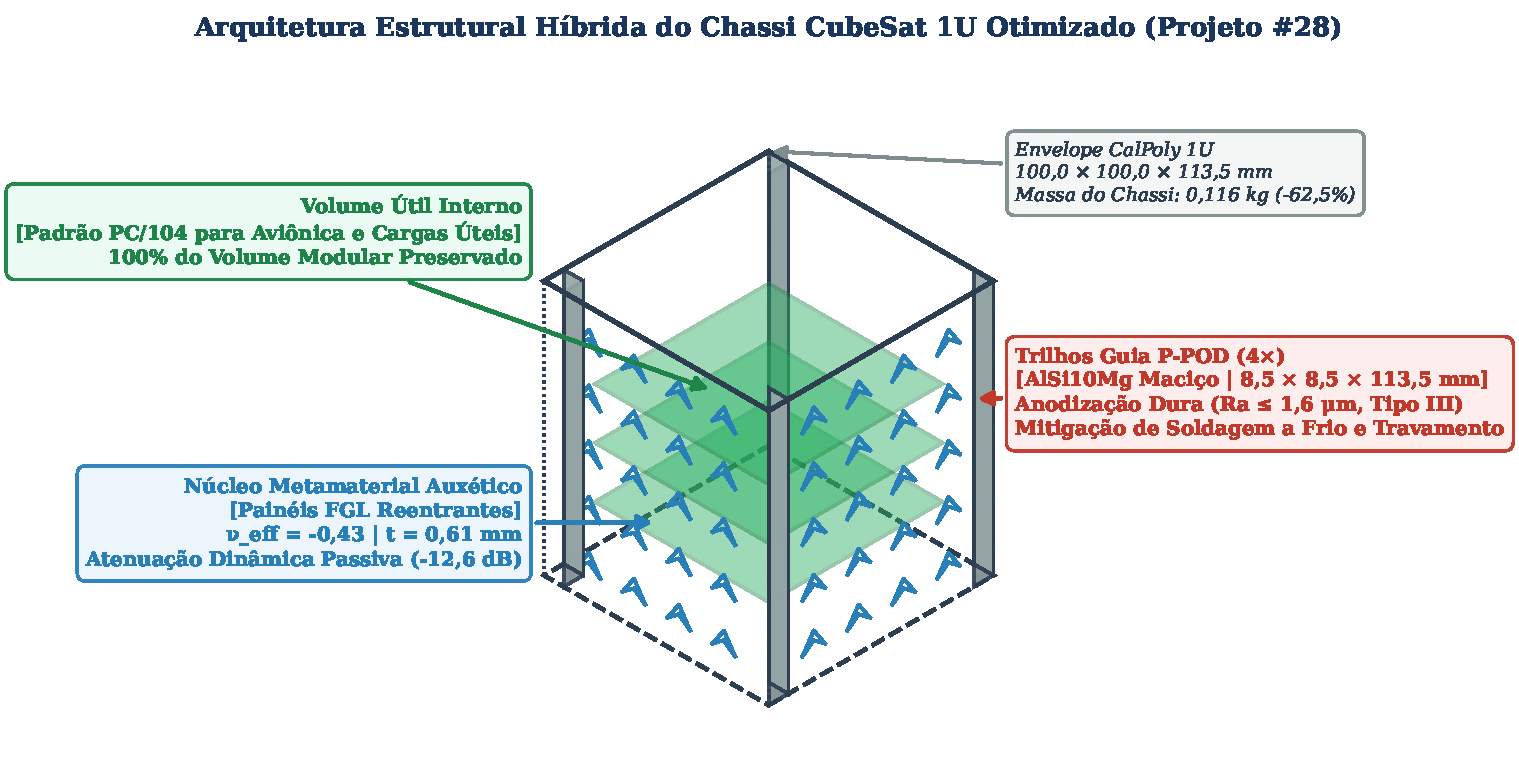
\includegraphics[width=0.82\textwidth]{./04-figuras/cubesat_1u_isometric_assembly}
  \fonte{Elaborada pelo autor (2026).}
\end{figure}

Chassis CubeSat 1U convencionais são historicamente fabricados como estruturas de alumínio usinado sólido (usualmente ligas das séries 6000 ou 7000). Embora apresentem facilidade de fabricação e rigidez estática adequada, essas soluções estruturais monolíticas impõem graves penalidades de engenharia:
\begin{alineas}
  \item \textbf{elevada massa estrutural passiva:} a estrutura metálica maciça consome tipicamente entre \SI{20}{\percent} e \SI{35}{\percent} do orçamento restrito de massa do CubeSat (cerca de \SI{300}{\gram} a \SI{350}{\gram}), subtraindo peso crítico que poderia ser destinado a baterias eletroquímicas, rodas de reação ou cargas úteis científicas;
  \item \textbf{alta transmissibilidade dinâmica e ressonância nociva:} por operarem sem amortecimento intrínseco significativo, estruturas convencionais atuam como condutores eficientes de energia vibratória, transmitindo níveis de aceleração estocástica de até \SI{12.0}{\Grms} diretamente para os módulos eletrônicos internos (padrão PC/104) e sensores de missão;
  \item \textbf{risco de falha funcional precoce:} dados epidemiológicos da base de dados orbital de nanossatélites (SWARTWOUT, 2023) indicam que mais de \SI{18}{\percent} das falhas em CubeSats decorrem de danos dinâmicos de lançamento, incluindo fadiga de soldas superficiais (BGA/SMD), desalinhamento de óptica e afrouxamento de fechos roscados estruturais.
\end{alineas}

Diante dessas restrições severas, surge a oportunidade tecnológica do emprego de \textbf{metamateriais mecânicos celulares auxéticos} (materiais com coeficiente de Poisson negativo, $\nu_{\text{eff}} < 0$) sintetizados em ligas metálicas aeroespaciais por \textbf{Manufatura Aditiva} via Fusão em Leito de Pó por Laser (\textit{Laser Powder Bed Fusion} -- L-PBF / SLM).

\section{Justificativa e relevância do trabalho}
\label{sec:justificativa}

Ao contrário dos materiais sólidos clássicos, que se expandem lateralmente sob compressão axial ($\nu > 0$), as microestruturas auxéticas com geometria reentrante contraem-se transversalmente quando comprimidas e expandem-se sob tração uniaxial. Essa cinemática interna singular confere às matrizes auxéticas propriedades físicas excepcionais:
\begin{enumerate}
  \item \textbf{rigidez específica elevada sob flexão celular:} capacidade de manter estabilidade mecânica sob espessuras de parede delgadas ($t < \SI{1.0}{\milli\metre}$);
  \item \textbf{blindagem dinâmica e isolamento mecânico passivo:} o desacoplamento modal e o descasamento de impedância mecânica entre o núcleo celular e os trilhos guia monolíticos deflagram mecanismos de antirressonância e confinamento de ondas elásticas de alta frequência (HUSSEIN; LEAMY; RUZZENE, 2014);
  \item \textbf{resistência superior ao cisalhamento e tenacidade à fratura:} mitigação de concentrações pontuais de tensão e elevação da dissipação de energia sem a necessidade de acoplamento de polímeros viscoelásticos externos, os quais sofrem degradação por desgaseificação (\textit{outgassing}) no vácuo espacial.
\end{enumerate}

A consolidação da manufatura aditiva metálica em liga de alumínio aeroespacial \textbf{AlSi10Mg} viabiliza a conformação direta de topologias celulares complexas com porosidade controlada. Entretanto, a aplicação dessa tecnologia em estruturas primárias de voo exige o cumprimento estrito dos requisitos de Projeto para Manufatura Aditiva (\textit{Design for Additive Manufacturing} -- DfAM), garantindo a ausência de suportes internos de impressão ($\theta_{\text{overhang}} \ge \SI{35.0}{\degree}$), integridade de poça de fusão laser ($t \ge \SI{0.50}{\milli\metre}$) e canais desobstruídos para evacuação de pó metálico residual ($\text{gap}_{\text{despoeiramento}} \ge \SI{1.50}{\milli\metre}$), em plena conformidade com as diretrizes da norma aeroespacial \textbf{NASA-STD-6030} (NASA, 2021).

\section{Problema de pesquisa e hipóteses de trabalho}
\label{sec:problema_hipoteses}

O problema central abordado neste trabalho pode ser formalizado na seguinte questão de engenharia:
\begin{quote}
  \itshape
  É possível conceber, otimizar e qualificar estruturalmente um chassi CubeSat 1U integrado por metamateriais celulares auxéticos em liga AlSi10Mg L-PBF que reduza substancialmente a massa estrutural passiva e atue simultaneamente como filtro mecânico protetor da carga útil, satisfazendo com folga as normas de rigidez, resistência e fadiga da NASA GEVS?
\end{quote}

Para responder a essa questão, estabelecem-se três hipóteses formais de trabalho:
\begin{alineas}
  \item \textbf{Hipótese 1 ($H_1$ -- Alívio mássico com preservação de rigidez):} A substituição dos painéis maciços por células auxéticas reentrantes de densidade graduada reduzirá a massa da estrutura primária em mais de \SI{40.0}{\percent} frente ao chassi monolítico usinado (\textit{baseline} de \SI{0.308}{\kilo\gram}), mantendo a primeira frequência natural fundamental estritamente acima do limite normativo aeroespacial ($f_1 \ge \SI{100.0}{\hertz}$);
  \item \textbf{Hipótese 2 ($H_2$ -- Isolamento dinâmico passivo da carga útil):} No regime sub-comprimento de onda ($a/\lambda \le \num{0.006} \ll 1$), o descasamento severo de impedância acústica ($Z_{\text{solid}} = \SI{13.47}{\mega\pascal\second\per\metre}$ versus $Z_{\text{eff}} = \SI{1.39}{\mega\pascal\second\per\metre}$, reflexão $> \SI{66}{\percent}$) e as antirressonâncias das costelas auxéticas proporcionarão atenuação de mais de \SI{50.0}{\percent} (superior a \SI{6.0}{\decibel}) na aceleração eficaz estocástica transmitida para a interface central da carga útil sob vibração aleatória NASA GEVS ($14{,}1\text{ G}_{\text{rms}}$);
  \item \textbf{Hipótese 3 ($H_3$ -- Eficiência de metamodelagem e confiabilidade à fadiga):} A integração de um modelo substituto neural guiado por física (\textit{Physics-Guided ResNet}) acelerará o ciclo de busca multiobjetivo (com \textit{speedup} instantâneo $> 100000\times$ e \textit{speedup} amortizado de ponta a ponta $\approx \num{40.0}\times$), convergindo para uma solução ótima com Margem de Segurança positiva ($MS_{\text{yield}} > 0$) e índice de dano por fadiga acumulada de Steinberg calculado de modo conservador no entalhe crítico amplamente abaixo do teto de qualificação espacial da NASA ($D \le \num{0.25}$), atingindo maturidade Digital TRL 4 (NASA SP-6105) e Hardware TRL 3 (ISO 16290:2013).
\end{alineas}

\section{Delimitação de escopo e rigor metodológico}
\label{sec:delimitacao}

Para resguardar a integridade técnica do trabalho, delimita-se categoricamente o escopo mecânico e material adotado:
\begin{enumerate}
  \item \textbf{modelo conceitual preliminar de interface (CAD / fit-check virtual):} geometrias conceituais impressas em filamento de Ácido Polilático (PLA) cumprem papel estritamente didático de verificação cinemática de montagem dos subsistemas, empacotamento volumétrico e interface com o dispensador P-POD. Em virtude do princípio de \textit{similaridade incompleta} (discrepâncias severas de módulo elástico, amortecimento histerético e comportamento térmico), os dados do polímero não são extrapolados para qualificação espacial de voo;
  \item \textbf{estrutura metálica de voo qualificada (liga aeroespacial AlSi10Mg L-PBF):} todas as simulações elastodinâmicas de alta ordem (Code\_Aster e CalculiX), a caracterização espectral PSD e o cálculo de dano de fadiga adotam as propriedades termomecanicamente consolidadas da liga de alumínio AlSi10Mg aliviada termicamente a \SI{300}{\celsius} por \SI{2}{\hour} ($E = \SI{68.0}{\giga\pascal}$, $\sigma_{\text{yield}} = \SI{230.0}{\mega\pascal}$, $\rho = \SI{2670.0}{\kilo\gram\per\cubic\metre}$).
\end{enumerate}

\section{Estrutura da monografia}
\label{sec:estrutura}

A presente monografia é estruturada em seis capítulos coesos:
\begin{itemize}
  \item \textbf{Capítulo 1 (Introdução):} contextualiza o tema, explicita o problema, as hipóteses de trabalho e a delimitação de escopo;
  \item \textbf{Capítulo 2 (Objetivos):} define o objetivo geral e os objetivos específicos estruturados nas quatro fases da pesquisa;
  \item \textbf{Capítulo 3 (Revisão da Literatura):} aborda a física dos metamateriais auxéticos, normas de vibração aleatória da NASA, princípios de DfAM metálico e fundamentos de modelos substitutos neurais;
  \item \textbf{Capítulo 4 (Metodologia):} descreve a esteira computacional aberta (OpenCASCADE, Gmsh Tet10, Code\_Aster, CalculiX), a arquitetura da rede neural informada por física e a otimização NSGA-II/TOPSIS;
  \item \textbf{Capítulo 5 (Resultados e Discussão):} analisa as topologias da fronteira de Pareto, a seleção do Projeto \#28, o estudo de convergência de malha pelo GCI de Roache, a blindagem dinâmica da carga útil, o cálculo de fadiga e o comparativo com a estrutura monolítica;
  \item \textbf{Capítulo 6 (Conclusão):} consolida os achados frente às hipóteses e propõe direcionamentos para trabalhos futuros.
\end{itemize}
